\section*{Результаты}
	
\addcontentsline{toc}{section}{Результаты}

	В итоге сделана программа для анализа периодических сигналов, поиска значимых гармоник и их аппроксимация для дальнейшего нахождения пика QPO. Также сравнены данные по MAXI J1820+070, полученные с инструментов Konus-Wind, Swift/BAT, INTEGRAL/ISGRI, что можно увидеть ниже. Интересно то, что, несмотря на одинаковый спектр регистрируемых фотонов у ISGRI и Konus-Wind, первый прибор после пика регистрировал больше фотонов, чем второй.
	
	\begin{figure}[h!]
		\begin{subfigure}[b]{0.45\textwidth}
			\centering
			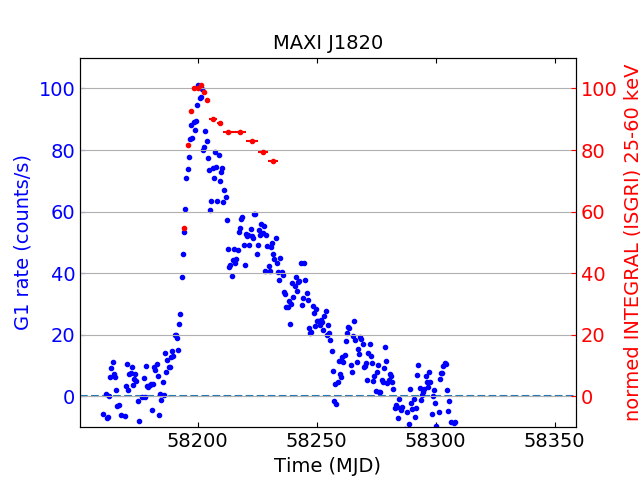
\includegraphics[width=\textwidth]{pictures/MAXIJ1820_kwG1_int.png}
			\caption{}
		\end{subfigure}
		\begin{subfigure}[b]{0.45\textwidth}
			\centering
			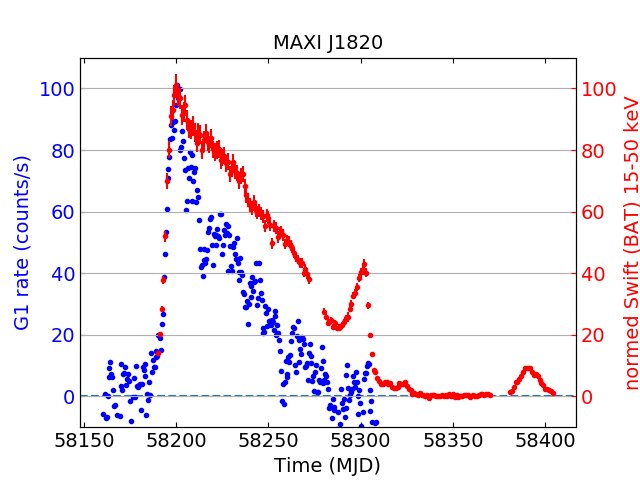
\includegraphics[width=\textwidth]{pictures/MAXIJ1820_kwG1_bat.png}
			\caption{}				
		\end{subfigure}
		\caption{Сравнение счета фотонов у Конус-Винд c (a) INTEGRAL или (b) BAT}
	\end{figure}
	
	Изначально была дана информация о первых 130 днях наблюдениия ха MAXI J1820+070. После разбиения сигнала на 130 однодневных сигналов, оказалось, что на 38-ой день в спектре мощности можно найти квазипериодические осцилляции. Их возможно обнаружить до 62 дня. Частота осцилляций увеличивалась со временем от $0{,}03$ до $0{,}078$ Гц.
	
	При построении графика зависимости частоты квазипериодических осцилляций от времени, получается, что ... (продолжение следует)

